%!TEX TS-program = XeLaTeX
%!TEX TS-program = XeLaTeX
\documentclass[11pt]{article}

\usepackage{amssymb}
\usepackage{amsthm}
\usepackage{amsmath}
\usepackage{mathtools}

\usepackage{fancyhdr}
\usepackage{graphicx}
\usepackage[top=3cm, left=2cm, right=2cm, headheight = 90pt]{geometry}
\usepackage{xltxtra}
\usepackage[font=small,labelfont=bf]{caption}

\usepackage{multicol}

\renewcommand{\theenumi}{\alph{enumi}}


\def\leq{\leqslant}
\def\geq{\geqslant}
\def\N{\mathbb N}
\def\R{\mathbb R}
\def\Z{\mathbb Z}
\DeclarePairedDelimiter\set\{\}

\def\prob{}

\theoremstyle{definition}
\newtheorem{problem}{\prob}


\pagestyle{fancy}

%!TEX TS-program = XeLaTeX

\fancyfoot[CE,CO]{}  % this is to remove page numbers (as you might want for single page docs)

%%!TEX TS-program = XeLaTeX
\renewcommand{\figurename}{Attēls}


\fancyhead[C]{{\Large\bf Graphs 1 - Problems}\\ \date}

\begin{document}

\noindent 
%\emph{\notes}

%1
\begin{problem}
\textit{[Bridges of Königsberg]}
City of Königsberg is located on both sides of the river Pregel and on two islands. There are seven bridges connecting islands as shown on Figure \ref{fig:sevenBridges}. Leonhard Euler wants to take a walk that would take him across each bridge exactly once. Can he do this? 
\begin{center}
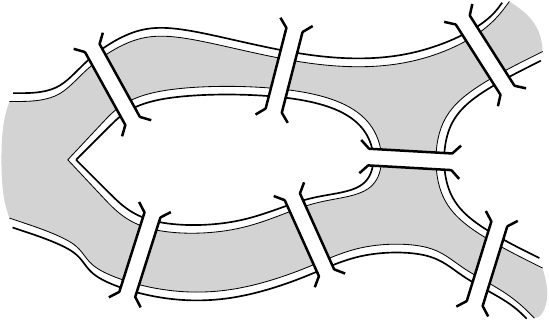
\includegraphics[width=4cm]{euler2.png}
\captionof{figure}{Seven bridges of Königsberg }
\label{fig:sevenBridges}
\end{center} 
\end{problem}
%

%2
\begin{problem}
\textit{[Weird classmates]}
A student once told James: "We have $35$ students in our class. And imagine - everyone has exactly $11$ friends within the class!". James, being good at Graph Theory, immediately replied that this is not possible. How did he know?
\end{problem}
%

%3
\begin{problem}
\textit{[Road planning]}
In the Kingdom of Wakanda there are $15$ towns and each of these are connected with direct roads with no less than $7$ other towns within this Kingdom. Prove that its possible to travel by road between any two towns (possibly via other towns)!
\end{problem}
%

%4
\begin{problem}
\textit{[Wire cube]}
Luize has a $120cm$ long piece of wire.
\begin{enumerate}
\item Can she make a cube with side length $10cm$ without cutting the wire?
\item If she does need to cut it, what is the minimum number of pieces?
\end{enumerate}
\end{problem}
%

%5
\begin{problem}
\textit{[Doodle]}
Is it possible to draw the picture from the Figure \ref{fig:doodle} without lifting pen from the paper?
\begin{center}
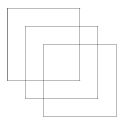
\includegraphics[width=3cm]{doodle.png}
\captionof{figure}{A doodle }
\label{fig:doodle}
\end{center} 
\end{problem}
%

%6
\begin{problem}
\textit{[Types of tournament]}
30 teams participated in the tournament. What was the total number of games they played, if:
\begin{enumerate}
\item All teams have to play each other
\item They do play-offs (in each game loser goes out, winner moves to next stage)
\end{enumerate}
\end{problem}
%

%7
\begin{problem}
\textit{[Circular reference]}
Edges of a regular polygon are marked with arrows (in one of the two possible directions). Prove that number of vertices which have two arrows going out of them is equal to number of vertices which have two arrows going into them!
\end{problem}
%

%8
\begin{problem}
\textit{[Forestry]}
A \textit{tree} is a set of nodes connected by sticks (each stick connecting exactly two nodes) where it is possible to travel between any two nodes (graph is connected), but it is not possible to travel somewhere and come back to original node not going though same stick twice (graph has no cycles).  A leaf is a node with just one stick connecting it. Prove that every tree has at least two leaves!
\end{problem}
%

%9
\begin{problem}
\textit{[Network robustness]}
What is the minimum number between of connections between $10$ information nodes to guarantee that if any two of them break down, the rest are still connected? 
\end{problem}
%


\end{document}
